\chapter{Overview}
\ac{ESSIG} is roughly composed out of three components. First we have
the input language, which can be used to describe the micro controller a
simulator should be generated for. Than we have a generator, which
creates an implementation of the private API (see VM) that the VM can
use in simulating the micro controller. Than we have our VM, in which
the micro controller will be simulated. It exposes a public API to a
client which can then simulate programs like they were running on the
simulator. The following diagram illustrates how the components relate
to each other.

\begin{center}
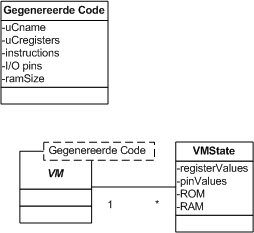
\includegraphics[width=5.376cm,height=4.932cm]{Essig-img002.png}
\end{center}

